\documentclass[a4paper,twoside]{ctexrep}

\ctexset{
	section = {
		format+ = \zihao{-4} \heiti \raggedright,
		name = {,、},
		number = \chinese{section},
		beforeskip = 1.0ex plus 0.2ex minus .2ex,
		afterskip = 1.0ex plus 0.2ex minus .2ex,
		aftername = \hspace{0pt}
	},
	subsection = {
		format+ = \zihao{5} \heiti \raggedright,
		name = {\thesubsection、},
		name = {,、},
		number = \arabic{subsection},
		beforeskip = 1.0ex plus 0.2ex minus .2ex,
		afterskip = 1.0ex plus 0.2ex minus .2ex,
		aftername = \hspace{0pt}
	}
}

\usepackage{blindtext}  
\usepackage{geometry}


% Page margin layout
\geometry{left=2.3cm,right=2cm,top=2.5cm,bottom=2.0cm}


\usepackage{listings}
\usepackage{xcolor}
\usepackage{geometry}
\usepackage{amsmath}
\usepackage{float}
\usepackage{hyperref}

\usepackage{graphics}
\usepackage{graphicx}
\usepackage{epsfig}
\usepackage{float}

\usepackage{algorithm}
\usepackage[noend]{algpseudocode}

\usepackage{booktabs}
\usepackage{threeparttable}
\usepackage{longtable}
\usepackage{listings}
\usepackage{tikz}
\usepackage{multicol}

\usepackage{caption}
\usepackage{subcaption}

% cite package, to clean up citations in the main text. Do not remove.
\usepackage{cite}

\usepackage{color,xcolor}

%% The amssymb package provides various useful mathematical symbols
\usepackage{amssymb}
%% The amsthm package provides extended theorem environments
\usepackage{amsthm}
\usepackage{amsfonts}
\usepackage{enumerate}
\usepackage{enumitem}
\usepackage{listings}

\usepackage{indentfirst}
\setlength{\parindent}{2em} % Make two letter space in the first paragraph
\usepackage{setspace}
\linespread{1.5} % Line spacing setting
\usepackage{siunitx}
\setlength{\parskip}{0.5em} % Paragraph spacing setting

% \usepackage[contents =22920202204622, scale = 10, color = black, angle = 50, opacity = .10]{background}

\renewcommand{\figurename}{图}
\renewcommand{\lstlistingname}{代码} 
\renewcommand{\tablename}{表格}
\renewcommand{\contentsname}{目录}
\floatname{algorithm}{算法}

\graphicspath{ {images/} }

%%%%%%%%%%%%%
\newcommand{\StudentNumber}{22920202204622}  % Fill your student number here
\newcommand{\StudentName}{\textbf{熊恪峥}\ 肖凯欣\ 谢哲涵\ 赵淇奥}  % Replace your name here
\newcommand{\PaperTitle}{基于xv6内核的网络子系统实现}  % Change your paper title here
\newcommand{\PaperType}{结题报告} % Replace the type of your report here
\newcommand{\Date}{2022年12月22日}
\newcommand{\College}{信息学院}
\newcommand{\CourseName}{计算机网络与通信}
%%%%%%%%%%%%%

%% Page header and footer setting
\usepackage{fancyhdr}
\usepackage{lastpage}
\pagestyle{fancy}
\fancyhf{}
% This requires the document to be twoside
\fancyhead[LO]{\texttt{\StudentName }}
\fancyhead[LE]{\texttt{\StudentNumber}}
\fancyhead[C]{\texttt{\PaperTitle }}
\fancyhead[R]{\texttt{第{\thepage}页,共\pageref*{LastPage}页}}


\title{\PaperTitle}
\author{\StudentName}
\date{\Date}

\lstset{
	basicstyle          =   \sffamily,          % 基本代码风格
	keywordstyle        =   \bfseries,          % 关键字风格
	commentstyle        =   \rmfamily\itshape,  % 注释的风格,斜体
	stringstyle         =   \ttfamily,  % 字符串风格
	flexiblecolumns,                % 别问为什么,加上这个
	numbers             =   left,   % 行号的位置在左边
	showspaces          =   false,  % 是否显示空格,显示了有点乱,所以不现实了
	numberstyle         =   \zihao{-5}\ttfamily,    % 行号的样式,小五号,tt等宽字体
	showstringspaces    =   false,
	captionpos          =   t,      % 这段代码的名字所呈现的位置,t指的是top上面
	frame               =   lrtb,   % 显示边框
}

\lstdefinestyle{PythonStyle}{
	language        =   Python, % 语言选Python
	basicstyle      =   \zihao{-5}\ttfamily,
	numberstyle     =   \zihao{-5}\ttfamily,
	keywordstyle    =   \color{blue},
	keywordstyle    =   [2] \color{teal},
	stringstyle     =   \color{magenta},
	commentstyle    =   \color{red}\ttfamily,
	breaklines      =   true,   % 自动换行,建议不要写太长的行
	columns         =   fixed,  % 如果不加这一句,字间距就不固定,很丑,必须加
	basewidth       =   0.5em,
}

\lstdefinestyle{MakefileStyle}{
	otherkeywords={.SUFFIXES},
	morekeywords={SUFFIX, CPP_,},
	moredelim=[is][\color{mbleu}]{/*}{*/},
	morecomment=[l][commentstyle]{\#},%
	emphstyle={\color{teal}},%
	moredelim=[s][\color{teal}]{\$(}{)}%
	basicstyle=\ttfamily\scriptsize\color{black!90},%
	stringstyle=\itshape\color{magenta},%
	showstringspaces=false,%
	keywordstyle=\bfseries\color{keycolor},%
	commentstyle=\color{blue}\slshape,%
	framexleftmargin=1mm,%
	backgroundcolor=\color{black!2},%
}

\lstdefinestyle{CppStyle}{
	language        =   c++,
	basicstyle      =   \zihao{-5}\ttfamily,
	numberstyle     =   \zihao{-5}\ttfamily,
	keywordstyle    =   \color{blue},
	keywordstyle    =   [2] \color{teal},
	stringstyle     =   \color{magenta},
	commentstyle    =   \color{red}\ttfamily,
	breaklines      =   true,   % 自动换行,建议不要写太长的行
	columns         =   fixed,  % 如果不加这一句,字间距就不固定,很丑,必须加
	basewidth       =   0.5em,
}

\algnewcommand\algorithmicinput{\textbf{Input:}}
\algnewcommand\algorithmicoutput{\textbf{Output:}}
\algnewcommand\Input{\item[\algorithmicinput]}%
\algnewcommand\Output{\item[\algorithmicoutput]}%

\usetikzlibrary{positioning, shapes.geometric}

% 流程图定义基本形状
\tikzstyle{startstop} = [rectangle, rounded corners, minimum width = 2cm, minimum height=1cm,text centered, draw = black]
\tikzstyle{io} = [trapezium, trapezium left angle=70, trapezium right angle=110, minimum width=2cm, minimum height=1cm, text centered, draw=black]
\tikzstyle{process} = [rectangle, minimum width=3cm, minimum height=1cm, text centered, draw=black]
\tikzstyle{decision} = [diamond, aspect = 3, text centered, draw=black]
% 箭头形式
\tikzstyle{arrow} = [->,>=stealth]

\newtheorem{assumption}{Assumption}[section]

\begin{document}
	
%%%%%%%%%%%%%%%%%%%%%%%%%%%%%%%%%%%%%%%%%%%%
\makeatletter % change default title style
\renewcommand*\maketitle{%
	\begin{center} 
		\bfseries  % title 
		{\LARGE \@title \par}  % LARGE typesetting
		\vskip 1em  %  margin 1em
		{\global\let\author\@empty}  % no author information
		{\global\let\date\@empty}  % no date
		\thispagestyle{empty}   %  empty page style
	\end{center}%
	\setcounter{footnote}{0}%
}
\makeatother
%%%%%%%%%%%%%%%%%%%%%%%%%%%%%%%%%%%%%%%%%%%%
	
	
\thispagestyle{empty}

\vspace*{1cm}

\begin{figure}[h]
	\centering
	
\includegraphics[width=4.0cm]{logo.png}
\end{figure}

\vspace*{1cm}

\begin{center}
	\Huge{\textbf{\PaperType}}
	
	\Large{\PaperTitle}
\end{center}

\vspace*{1cm}

\begin{table}[h]
	\centering	
	\begin{Large}
		\renewcommand{\arraystretch}{1.5}
		\begin{tabular}{p{3cm} p{5cm}<{\centering}}
			姓\qquad 名 & \StudentName  \\
			\hline
			学\qquad号 & \StudentNumber \\
			\hline
			日\qquad期 & \Date  \\
			\hline
			学\qquad院 & \College  \\
			\hline
			课程名称 & \CourseName  \\
			\hline
		\end{tabular}
	\end{Large}
\end{table}

\newpage

\title{
	\Large{\textcolor{black}{\PaperTitle}}
}
	
	
\tableofcontents

% 1.项目名称+项目组成员(分工)
% 2.项目背景/动机/目标
% 3.项目内容/任务/方案
% 4.结果和分析--可与3合起来撰写(试情况而定)
% 5.实验小结/感想
% 附件:相关代码文档、文件记录、PPT、视频文件(如果有的话)
% 建议报告和所有附件打包上传
 
\newpage
\setcounter{page}{1}

\begin{spacing}{1.2}

\chapter{分工}

\begin{table}[h]
	\centering
	\caption{成员及分工}
	\label{tbl:work}
	\renewcommand\arraystretch{1.5}
	\begin{tabular}{|c|p{0.8\textwidth}|}
		\toprule
		\hline
		成员 & 分工 \\
		\hline
		熊恪峥 & 项目总体设计、PCI和网卡驱动程序、Socket API和POSIX NetDB API编写、用户库支持、更先进的内存管理和文件系统支持的实现、daytime程序编写\\
		\hline
		肖凯欣 & ping/traceroute命令实现 \\
		\hline
		赵淇奥 & nslookup命令实现 \\
		\hline
		谢哲涵 & httpget命令实现 \\
		\hline
		\bottomrule
	\end{tabular}

\end{table}

\chapter{项目介绍}

\section{选题介绍}

由6.828 Lab 6\cite{kaashoek20066}得到的灵感,我们将为xv6内核实现完整的网络子系统以及相应的API。

6.828课程中讲授xv6内核\cite{cox2011xv6}的实现,并在实验中要求学生在称之为JOS的实验性微内核
操作系统中添加相应的功能。但事实上,xv6内核本身的结构和现代网络服务器中常常使用
的Linux和FreeBSD更为类似。因此,我们好奇,我们是否可以对xv6内核进行修改,来添加
对网络功能的支持,而不是在JOS上进行实现。这样,我们能够更好地通过实现相应的功能和
适配相应的库来加深对各种网络协议以及Socket API本身的理解。


\subsection{xv6简介}

xv6是对Dennis Ritchie's and Ken Thompson的Unix
Version 6 (v6)的重新实现。xv6与v6有大致相同的结构和代码风格,
但是使用了ANSI C实现,并且为现代的处理器功能,如对称多核心等做出了相应的适配。
它主要为MIT的操作系统教学而设计。

\subsection{lwIP简介}

lwIP\cite{dunkels2001design}是一个开源的、轻量级的TCP/IP协议栈,它是一个可移植的、可裁剪的、可靠的、高效的、低成本的TCP/IP协议栈,它可以用于嵌入式系统,如微控制器、单片机、DSP等。
lwIP最初是由Swedish Institute of Computer Science的Adam Dunkels开发,现在由开源社区开发和维护。并且被多个技术公司用于商业产品中,
如Intel/Altera, Analog Devices, Xilinx, TI, ST 和 Freescale。

\section{项目内容}

为了实现完整的网络子系统,我们需要实现以下内容:

\begin{itemize}
	\item 网卡驱动程序
	\item IP协议栈
	\item Socket API等应用编程接口支持、DNS等辅助功能的支持
	\item 用户库支持、网络应用程序
	\item 操作系统内核其他组件的增强
\end{itemize}

因此,我们首先实现了Intel e1000网卡的驱动程序。该设备被模拟器QEMU较好地支持,因此易于测试。为了使该设备
能够正常运行,需要实现PCI总线的支持。然后,我们移植了LWIP作为IP协议栈,它提供包括IP、ICMP、UDP和TCP协议的支持。
为了支持该库的正常运行,我们实现了相应的时钟中断处理程序及其各组件的初始化。基于该协议栈,我们首先提供了
以Socket API为代表的网络编程接口的支持,然后实现了以符合POSIX标准的\texttt{gethostbyaddr}和\texttt{gethostbyname}
为接口DNS的支持。最后,我们实现了包括基础的TCP/UDP Echo Server、例如nslookup、ping、traceroute、httpget等常见的实用程序,
以及符合RFC 867的日期时间协议的授时客户端。

此外,在开发过程中,我们严格采用了版本控制系统Git,以便于团队成员之间的协作开发。在开发流程上,我们坚持通过fork/pull request的方式进行代码的提交和合并,
以保证代码的质量、防止不当更改损坏项目的其他部分。我们的工作流程和现代的软件开发工作流程高度一致、完全接轨。实现了有效的
项目管理。在开发过程中,我们严格遵循了谷歌开源项目风格指南的代码规范,以保证代码的可读性和可维护性。

我们在开发结束后贯彻“从开源中来、到开源中去”的理念,将我们的项目以MIT协议开源,以供其他人参考和使用。项目地址是\url{https://github.com/SmartPolarBear/xv6_enhanced}

\chapter{项目实现}

\section{总体架构}
总体的项目架构如图~\ref{fig:arch}所示。
\begin{figure}[htb]
	\centering
	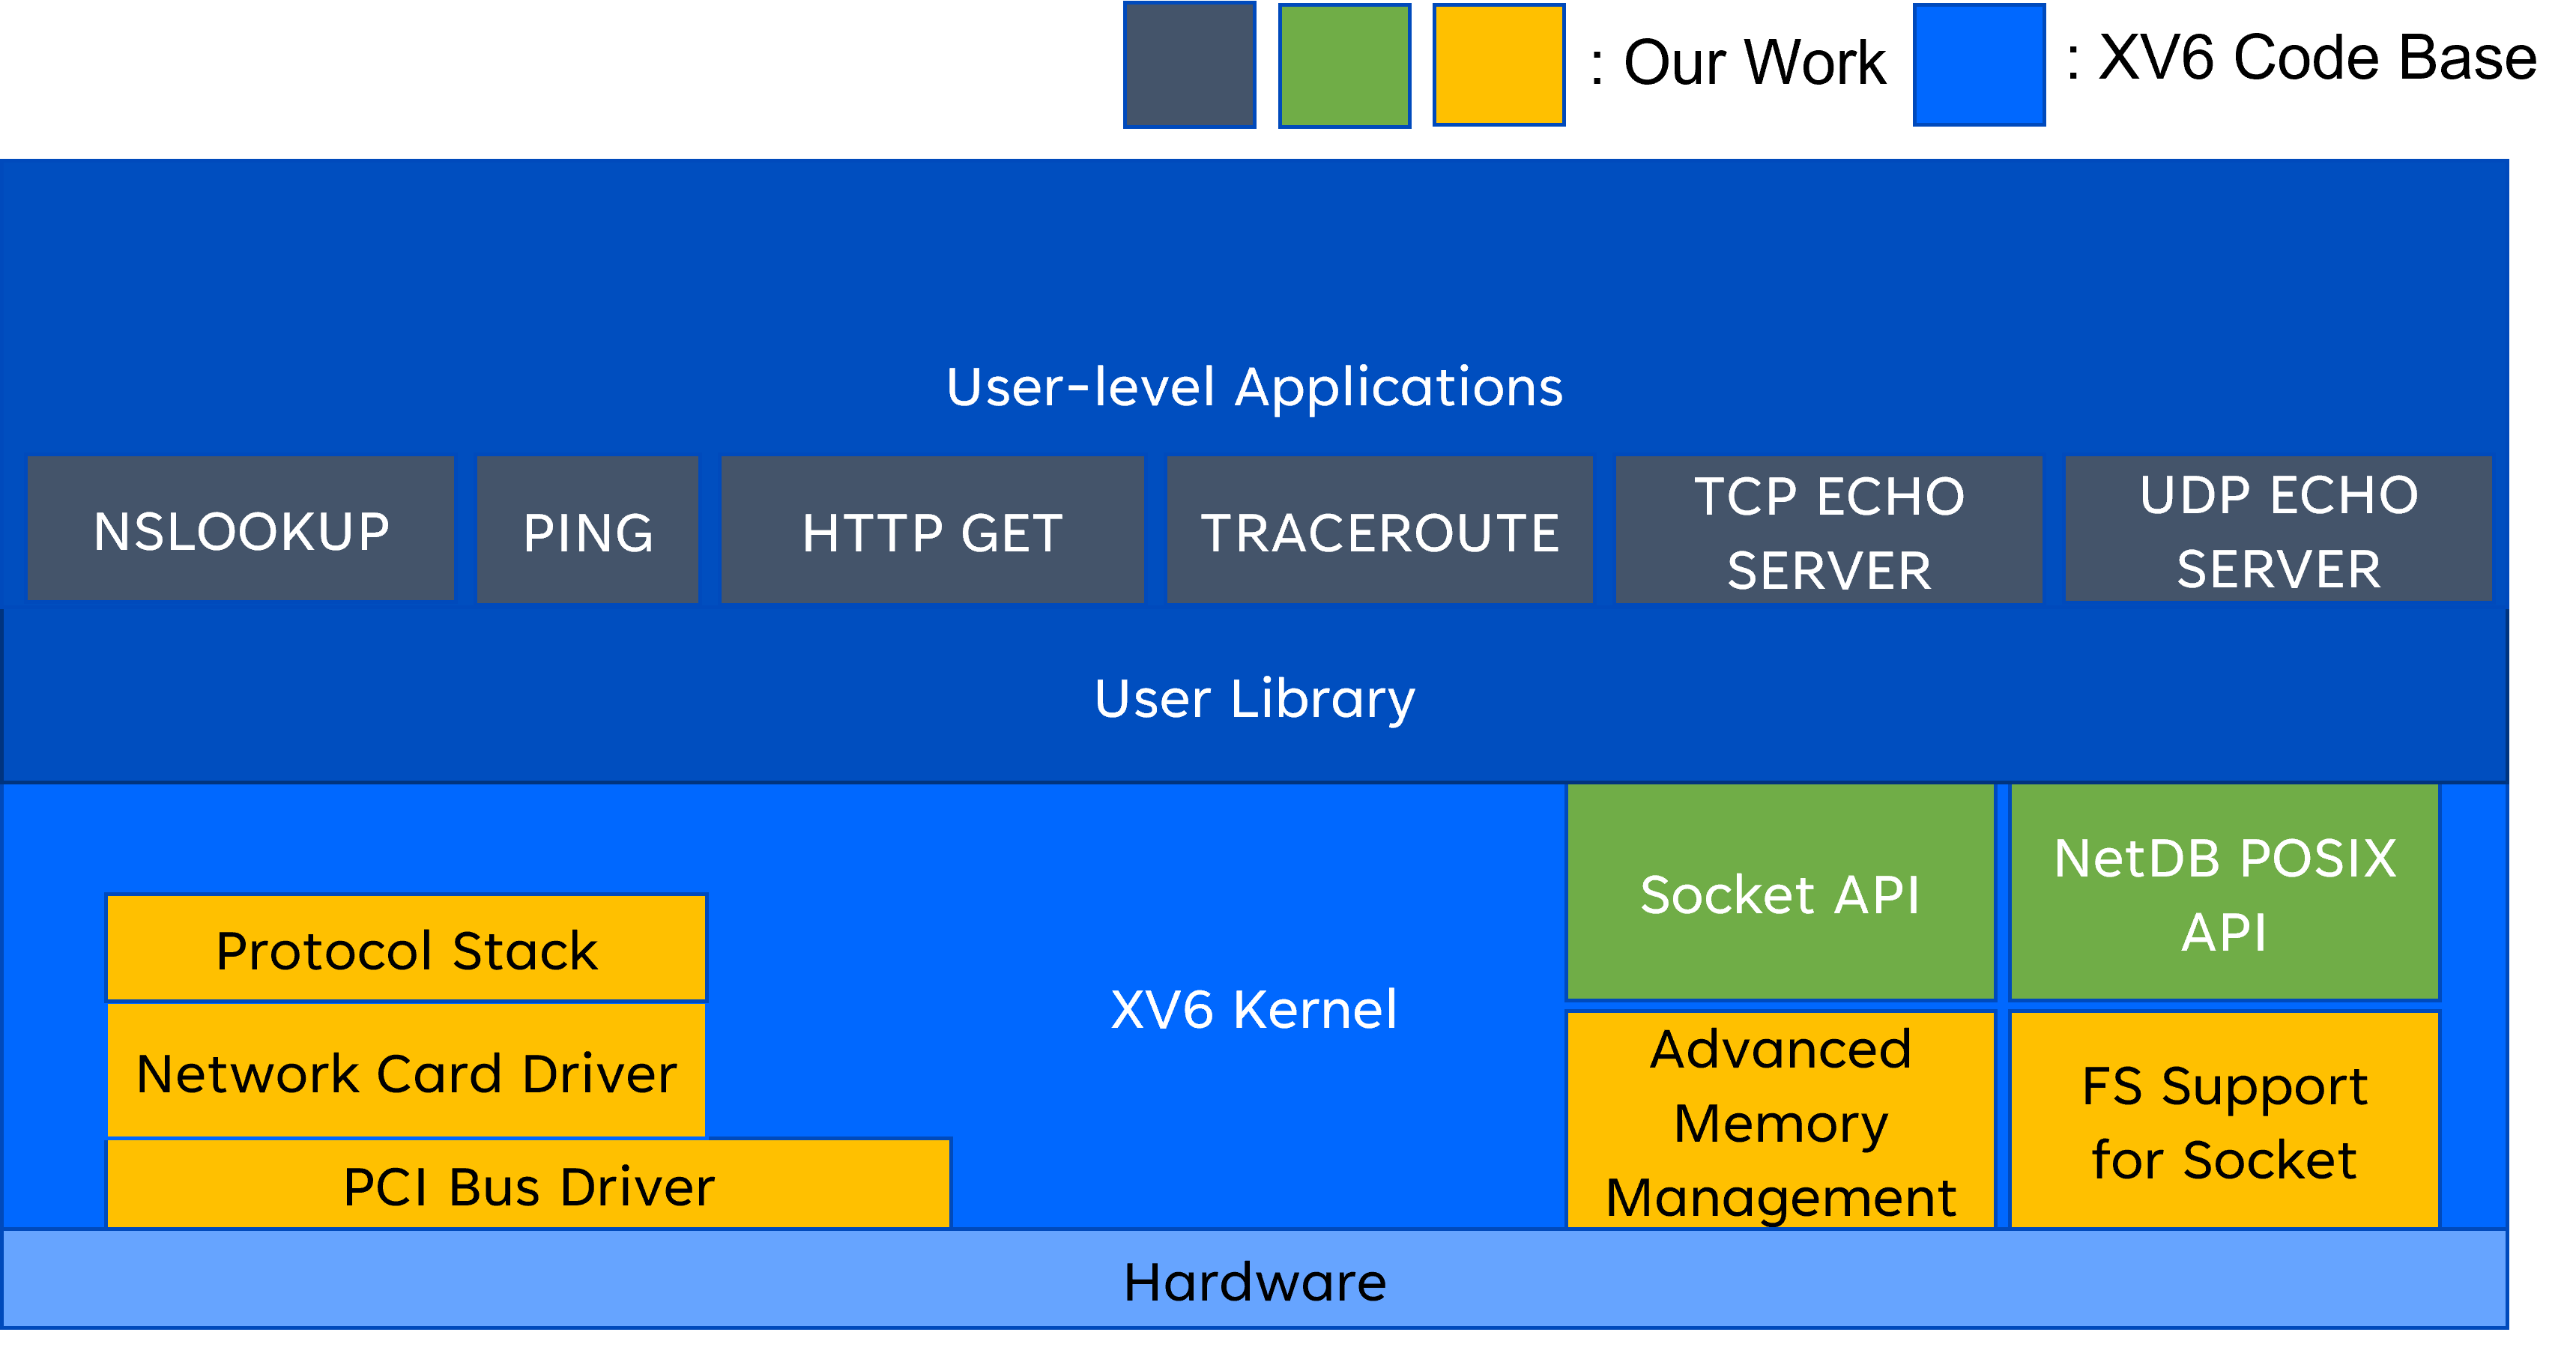
\includegraphics[width=0.8\textwidth]{arch.png}
	\caption{项目架构}
	\label{fig:arch}
\end{figure}

在内核态中的部分按功能分,可以分为三个部分:

一是负责处理实际数据收发、通讯的部分,自下而上分别是PCI总线的驱动、e1000网卡的驱动程序、基于LWIP的网络协议栈。
二是作为向上层提供服务的部分,包括提供一套数据收发原语的Socket API、提供一套使用DNS服务的接口的POSIX NetDB API部分。
三是围绕网络子系统内存分配频繁、动态内存分配要求高的需求、Socket API与类UNIX操作系统的文件系统部分结合紧密的特点,对内核进行的改进。
例如对内存分配的改进、对文件系统的改进、引入了与Linux内核中实现方式类似的链表等基础数据结构。

在内核和用户之间,用户态库也需要进行相应接口的实现。我们实现了Socket API和用于查询DNS的接口,例如
\texttt{gethostbyaddr}和\texttt{gethostbyname}的用户态库接口。
这些接口完全符合POSIX标准。

在用户态,我们实现了两类的应用程序:

第一类是用来调试、检验基础功能的应用程序。包括TCP、UDP的Echo Server、测试和远程主机实际通信以及DNS的
RFC 867日期时间服务客户端。
第二类是常用的网络实用程序,包括nslookup、ping、traceroute、httpget等。

\section{设备驱动程序的实现}

\subsection{PCI总线的驱动}

通用串行总线(PCI)是一种用于确保高性能、低开销的传输的本地总线。PCI总线的组件和卡片接口时处理器无关的,
因此该总线结构可以被多种处理器架构利用。

为了初始化PCI总线,需要驱动程序访问PCI配置空间,从而获取PCI设备的基本信息,例如设备的ID、设备的基地址等。
访问PCI配置空间有两种方式,但只有访问I/O端口的方式是符合标准的。这种方式使用两个32位的I/O端口,一个用于
指定配置地址,一个用于读写配置数据。配置地址的格式如图~\ref{fig:pci_config_addr}所示。
\begin{figure}[htb]
	\centering
	\caption{PCI配置地址的格式}
	\label{fig:pci_config_addr}
	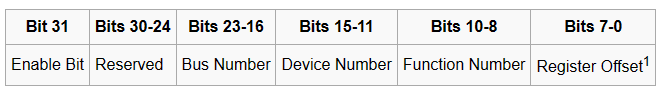
\includegraphics[width=0.5\textwidth]{controlreg.png}
\end{figure}
据此,我们实现的PCI驱动程序在代码\texttt{kernel/pci.c}中,它会访问PCI配置空间,获取PCI设备的基本信息,然后
加入设备表中。为了保证该驱动程序的可扩展性,我们的实现将不同驱动程序实现的相应初始化程序注册到数组中,如代码~\ref{code:pcireg}。
\begin{lstlisting}[numbers=left,style=CppStyle,caption={PCI驱动程序的初始化程序注册},label={code:pcireg}]
struct pci_driver pci_attach_vendor[] = {
	{0x8086, 0x100e, &e1000_nic_attach},
	{0x1af4, 0x1000, &virtio_nic_attach},
	{0, 0, NULL},
};
\end{lstlisting}
当驱动程序初始化的时候,每当注册新设备,都会在其中查找相应的初始化程序,然后调用该初始化程序。查找的方式
是读取设备类和设备ID,分别位于配置空间的偏移0x0b和0x0a中。如果找到相应的初始化程序,就调用该初始化程序。

当PCI驱动程序完成后,操作系统启动时,会调用\texttt{pci\_init}函数,该函数会遍历所有的PCI设备,完成
上述功能,并输出设备的基本信息。输出的信息如图~\ref{fig:initpci}所示。
\begin{figure}[htb]
	\centering
	\caption{PCI设备的基本信息}
	\label{fig:initpci}
	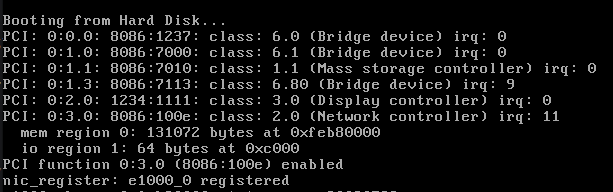
\includegraphics[width=0.5\textwidth]{initpci.png}
\end{figure}


\subsection{e1000网卡的驱动程序}

有了上述PCI驱动程序和相应扩展架构的实现。我们就可以实现e1000网卡的驱动程序了。e1000网卡的驱动程序的
重要组成部分是网卡的初始化程序,该程序会初始化网卡的寄存器,设置相应信息,使网卡进入可用状态。

\subsubsection{网卡的初始化}

有了完善的PCI驱动程序,e1000网卡的初始化在操作上就是对相应寄存器地址的读写。方法是调用PCI驱动程序
的\texttt{pciw}和\texttt{pcir}函数,分别用于写和读。

\section{基于LWIP的网络协议栈}

\section{Socket API}

\section{POSIX NetDB API和DNS解析}

\section{内核改进}

\subsection{内存分配改进}

原始的xv6内核中,内存分配只有\texttt{kalloc}和\texttt{kfree}两个函数,分别用于分配和释放内核内存。该
函数的作用是按页分配内存,每次分配的内存大小为一页,即4KB。这种分配方式存在两个问题:
\begin{enumerate}
	\item 由于每次分配的内存大小为一页,因此分配的内存大小不可控,如果需要分配的内存大小不是一页的整数倍,那么就会造成内存浪费。
	\item 当分配超过一页时,难以保证分配的内存是连续的。
\end{enumerate}
然而,在网络驱动程序、网络协议栈、Socket API等部分,需要频繁地进行内存分配,而且分配的内存大小不固定、分配的大小常常远小于
4KB。为了避免耗尽内存,提高内存分配的效率。需要改进内存分配的方式。

常见的类UNIX操作系统,例如Linux有更加复杂的内存分配机制。例如Buddy/Slab分配器,可以分配任意大小的内存块。其中Buddy分配器
分配2幂次大小的内存块,而Slab分配任意指定大小的内存块。这种分配方式的优点是可以分配任意大小的内存块,然而完整的实现相当复杂,
不利于我们按期完成项目。因此,我们采用了一种简单的内存分配方式,即利用xv6现有的分配器分配页大小的内存。然后使用Slab分配器
分配任意大小的内存块。具体的实现在\texttt{kernel/slab.c}中。

Slab分配器的原理是将内存分为多个大小相同的内存块,每个内存块称为一个Slab。Slab分配器维护一个Slab链表,每个Slab中都有一个
空闲链表,用于记录空闲的内存块。当需要分配内存时,Slab分配器从空闲链表中取出一个内存块,当需要释放内存时,Slab分配器将内存块
插入空闲链表。当Slab中的内存块全部被分配时,Slab分配器从Slab链表中取出一个Slab,当Slab中的内存块全部被释放时,Slab分配器
将Slab插入Slab链表。它们操作的内存空间均由xv6的分配器分配。

我们的实现接口大致于Linux相应组件的接口相同。\texttt{kernel/slab.h}中定义了Slab的存储结构,如代码~\ref{code:slab}所示。
\begin{lstlisting}[numbers=left,style=CppStyle,caption={Slab的存储结构},label={code:slab},language=C]
typedef struct slab
{
	kmem_cache_t *cache;
	size_t in_use;
	size_t next_free;
	void *objects;
	kmem_bufctl *bufctl;

	spinlock_t lock;

	list_head_t link;
} slab_t;
\end{lstlisting}
而这些Slab由称之为Cache的结构管理。Cache的存储结构如代码~\ref{code:cache}所示,在\texttt{kernel/include/slab.h}中。
\begin{lstlisting}[numbers=left,style=CppStyle,caption={Cache的存储结构},label={code:cache},language=C]
typedef struct kmem_cache
{
	list_head_t full, partial, free;

	list_head_t link;

	size_t obj_size, obj_count;
	uint flags;
	spinlock_t lock;

	char name[KMEM_CACHE_NAME_MAXLEN];
} kmem_cache_t;
\end{lstlisting}
有了这些结构,我们就可以实现\texttt{kmem\_cache\_create}、\texttt{kmem\_cache\_alloc}、\texttt{kmem\_cache\_free}等接口。

在这些接口之上,我们也实现了\texttt{kmalloc},来方便不创建对应Cache,只指定大小的内存分配。
这些接口在驱动程序、Socket API和DNS相关的实现中发挥了关键的作用。


\subsection{文件系统改进}

xv6没有常见的VFS结构,但是其文件系统实现包含了对不同类型的文件节点的初步支持。
由于Socket API在分配、关闭Socket时需要创建相应类型的文件节点来返回File Descriptor,
因此我们在xv6的文件系统实现上做了一些扩展。

\texttt{kernel/fs.h}中定义了文件节点的存储结构,如代码~\ref{code:file}所示。
\begin{lstlisting}[numbers=left,style=CppStyle,caption={文件节点的存储结构},label={code:file},language=C]

typedef enum file_type
{
	FD_NONE = 1,
	FD_PIPE,
	FD_DEVICE,
	FD_SOCKET,
} file_type_t;

typedef struct file
{
	file_type_t type;
	int ref; // reference count
	char readable;
	char writable;

	union
	{
		struct pipe *pipe;
		struct inode *ip;
	};
	uint off;
}file_t;

\end{lstlisting}
我们在类型中加入了\texttt{FD\_SOCKET},并在\texttt{union}中加入了\texttt{socket}成员。
这样就存储了Socket的相关信息。

负责处理文件节点的函数包括\texttt{file\_alloc}、\texttt{file\_close}、\texttt{file\_dup}等。
我们在相应函数中加入了对Socket的处理,调用Socket相关的具体实现,这里举一例说明,如代码~\ref{code:fileclose}所示。
\begin{lstlisting}[numbers=left,style=CppStyle,caption={file\_alloc函数的修改},label={code:fileclose},language=C]
void
fileclose(struct file *f)
{
	struct file ff;

	acquire(&ftable.lock);
	if (f->ref < 1)
	{
		panic("fileclose");
	}
	if (--f->ref > 0)
	{
		release(&ftable.lock);
		return;
	}
	ff = *f;
	f->ref = 0;
	f->type = FD_NONE;
	release(&ftable.lock);

	if (ff.type == FD_PIPE)
	{
		pipeclose(ff.pipe, ff.writable);
	}
	else if (ff.type == FD_INODE)
	{
		begin_op();
		iput(ff.ip);
		end_op();
	}
	else if (ff.type == FD_SOCKET)
	{
		socketclose(ff.socket);
	}
}
\end{lstlisting}

在这段代码中,遇到Socket类型的文件节点时,调用了\texttt{socketclose}函数
实现Socket专属的关闭逻辑。

\subsection{常用数据结构实现}

设备驱动程序、DNS的查询过程中,我们需要一些能够动态地插入和删除元素的数据结构。
因此,我们实现了Linux类似的侵入式链表。

侵入式(Intrusive)链表是一种链表的实现方式,它将链表的节点单独定义为一个结构体,
并将链表节点的指针作为结构体的成员,这是链表中相应的指针都处于数据的内部,所以称之为侵入式链表。

这种链表实现的好处在于可以用同一套链表操作函数来操作不同的具体数据。当需要从链表节点获取数据时,
可以通过结构体中内存偏移的计算来获取数据的指针,从而实现链表节点和数据的互相获取。
这种计算的方法在Linux内核中被称为\texttt{container\_of}。代码~\ref{code:containerof}给出了这种计算的实现。

\begin{lstlisting}[numbers=left,style=CppStyle,caption={container\_of宏的实现},label={code:containerof},language=C]
// offset of a struct member
#define offsetof(type, member)  __builtin_offsetof (type, member)

// get struct pointer from member
#define container_of(ptr, type, member) ({                      \
        const typeof( ((type *)0)->member ) *__mptr = (ptr);    \
        (type *)( (char *)__mptr - offsetof(type,member) );})
\end{lstlisting}

而其余的链表操作函数实现定义在\texttt{include/list.h}中。包括插入、删除、遍历等操作。
这些操作函数的实现都是基于\texttt{list\_head}结构体的。

\section{用户态库}

用户态库是用户态和系统调用实现间的“胶水”。它对用户提供了POSIX兼容的编程接口。将相关参数
按照系统调用的约定存入内存,然后调用INT 0x80中断,将控制权交给内核。用户态库的实现在
\texttt{lib/ulib}目录下。

由于在32位环境下,传参数不会用到寄存器,因此已经正确地将参数存入内存中,只需要使用int指令
调用相应终端即可,这部分代码实现在\texttt{lib/ulib/usys.S}中。如代码~\ref{code:usys}所示。
\begin{lstlisting}[numbers=left,style=CppStyle,caption={usys.S中的系统调用实现},label={code:usys}]
#define SYSCALL(name) \
  .globl name; \
  name: \
    movl $SYS_ ## name, %eax; \
    int $T_SYSCALL; \
    ret
\end{lstlisting}
这定义了一个宏,用于定义系统调用的实现。宏中的\texttt{SYS\_name}是系统调用的编号,\texttt{T\_SYSCALL}是中断号。

这样就可以简单地用系统调用的名称迅速定义大量的系统调用库函数接口了。


\section{应用程序}

\subsection{nslookup}

\subsubsection{程序介绍}

nslookup是一个用来查询因特网域名服务器的程序。程序允许使用者向域名服务器查询一个域名或
地址的信息,通常被用来诊断域名解析系统的基本结构信息,查询域名解析是否正常工作,在网络
故障时排查网络问题。

\subsubsection{功能分析}

一个完整的nslookup程序拥有两种使用模式:交互式与⾮交互式。
交互式的nslookup允许用户交互式查询多个主机/域名信息,并且具有多种交互命令用于处理复杂的
需求、提升用户体验。而⾮交互式的nslookup只允许用户一次性查询单个主机/域名信息。⾮交互式
的nslookup也⽀持通过命令⾏指定参数。
本项⽬的⽬标是实现一个简易的nslookup程序,因此此程序只实现了nslookup的核⼼功能:⾮交互
式地对域名或地址进⾏查询,并向用户显示查询结果。

\subsubsection{程序实现}

在本项目开始时,我尝试通过如下方法实现程序的查询功能:
\begin{enumerate}
	\item 通过socket编程与域名服务器通信
	\item 构造DNS QUERY报文,向域名服务器发起域名查询请求
	\item 解析DNS RESPONSE报文,解析由域名服务器返回的主机信息
\end{enumerate}

但是该方法⾯对的最大的障碍是,由于DNS复杂的压缩规则,通过编程解析DNS REPLY报文实现难
度较⾼。

因此我最后通过调用内核中已经实现的函数:gethostbyname与gethostbyaddr,获得主机信息。内
核中,netdb.h中实现了一组用来获取主机信息的函数,其中包括gethostbyname与
gethostbyaddr。这组函数会返回一个保存有主机信息的hostent结构体。
其定义如下代码~\ref{code:hostent}所示。

\begin{lstlisting}[numbers=left,style=CppStyle,caption={hostent结构体定义},label={code:hostent}]
	struct  hostent { 
             char    *h_name;        /* official name of host */ 
             char    **h_aliases;    /* alias list */ 
             int     h_addrtype;     /* host address type */ 
             int     h_length;       /* length of address */ 
             char    **h_addr_list;  /* list of addresses from name 
server */ 
     }; 
\end{lstlisting}
   
程序具体实现如下:
\begin{enumerate}
	\item 首先通过命令行接受用户输入参数,并对用户输入作初步的输入检查
	\item 对于用户的输入,使用inet\_pton判断输入类型,对地址和域名分别处理
	\item 对于输入的域名,通过调用gethostbyname获取描述该主机的hostent结构体
	\item 对于输入的地址,通过调用gethostbyaddr获取描述该主机的hostent结构体
	\item 对于获取的hostent结构体,使用用户友好的形式输出显示。
\end{enumerate}


\subsection{ping和traceroute}

\subsubsection{ping的实现}

利用原始套接字发送ICMP报文,将ICMP报文头的消息类型设置为8(ICMP request)。
ICMP\_HDR报文头如代码~\ref{code:ICMPHDR}所示。

\begin{lstlisting}[numbers=left,style=CppStyle,caption={ICMP\_HDR结构体定义},label={code:ICMPHDR}]
struct icmp_hdr {
	unsigned char type;		/* message type */
	unsigned char code;		/* type sub-code */
	unsigned short checksum;
	unsigned short id;
	unsigned short sequence;
	unsigned int timestamp;		/* not part of ICMP, but we need it */
};
\end{lstlisting}

然后,通过原始套接字实现的ICMP报文的发送,如代码~\ref{code:sendICMP}所示。

\begin{lstlisting}[numbers=left,style=CppStyle,caption={ICMP报文发送函数},label={code:sendICMP}]
struct sockaddr_in dest;
dest.sin_family = AF_INET;
dest.sin_port = htons(0);
dest.sin_addr.s_addr = ip;
char buff[sizeof(ICMP_HDR) + 32];
ICMP_HDR *pIcmp = (ICMP_HDR *) buff;
pIcmp->icmp_type = 8; 
pIcmp->icmp_code = 0;
pIcmp->icmp_id = (uint16_t) pID;
pIcmp->icmp_checksum = 0;
pIcmp->icmp_sequence = 0;
memset(&buff[sizeof(ICMP_HDR)], 'E', 32);
\end{lstlisting}

然后解析接收到的ICMP报文,判断是否为ICMP reply,如果是,则计算往返时间,否则丢弃并报错。
如代码~\ref{code:recvICMP}所示。
\begin{lstlisting}[numbers=left,style=CppStyle,caption={ICMP报文接收函数},label={code:recvICMP}]
ICMP_HDR *pRecvIcmp = (ICMP_HDR *) (recvBuf + 20); // (ICMP_HDR*)(recvBuf + sizeof(IPHeader));
IPHeader *ipHeader = (IPHeader *) recvBuf;
\end{lstlisting}
其中IPHeader结构体定义如代码~\ref{code:IPHeader}所示。
\begin{lstlisting}[numbers=left,style=CppStyle,caption={IPHeader结构体定义},label={code:IPHeader}]
	typedef struct IPHeader {
    uint8_t iphVerLen; 
    uint8_t ipTOS; 
    uint16_t ipLength; 
    uint16_t ipID; 
    uint16_t ipFlags; 
    uint8_t ipTTL; 
    uint8_t ipProtocol;
    uint16_t ipChecksum;
    uint32_t ipSource; 
    uint32_t ipDestination; 
} IPHeader;
\end{lstlisting}
由此可以显示相应的信息,如代码~\ref{code:ping}所示。
\begin{lstlisting}[numbers=left,style=CppStyle,caption={ping显示信息},label={code:ping}]
printf(" %d bytes from %s:", (int) nRet, inet_ntoa(from.sin_addr));
printf(" icmp_seq = %d. ", pRecvIcmp->icmp_sequence);
printf(" ttl = %d. ", ipHeader->ipTTL);
printf(" time: %d ms", (int) nTick - (int) pRecvIcmp->icmp_timestamp);
\end{lstlisting}

\subsubsection{traceroute的实现}

与ping类似,traceroute从1开始设置ttl,当报文每经过一个路由节点时,ttl减小1,当ttl为0时,节点丢弃报文,并向主机发送一个超时报文,报文的ip数据报中就有该节点的ip地址;随后增大ttl,获取下一个节点,就可以得知主机和目的地址之间的所有路由节点的ip地址

但是,因为部分节点不会响应icmp报文,发送超时报文,所以要为套接字设置超时。其中设置超时的代码如代码~\ref{code:settimeout}所示。
\begin{lstlisting}[numbers=left,style=CppStyle,caption={设置超时},label={code:settimeout}]
struct timeval timeout = {5,0};
setsockopt(sRaw,SOL_SOCKET,SO_RCVTIMEO,(char *)&timeout,sizeof(struct timeval));
\end{lstlisting}
而设置ttl的代码如代码~\ref{code:setttl}所示。
\begin{lstlisting}[numbers=left,style=CppStyle,caption={设置TTL},label={code:setttl}]
	setsockopt(sRaw, IPPROTO_IP, IP_TTL, &ttl, sizeof(ttl))
\end{lstlisting}

\subsection{httpget}

\subsection{RFC 867授时服务客户端daytime}

Daytime Protocol是1983年由RFC 867定义的,用于授时服务,客户端通过TCP连接或者到服务器,服务器
使用的端口号是13,服务器返回一个ASCII字符串,表示当前的时间,格式为:$Day Mon dd hh:mm:ss yyyy$

为了测试与远程服务器的连接,我们可以使用这个协议,客户端的代码如代码~\ref{code:datetime}所示。
该实现使用Socket编程,使用了TCP连接,连接到服务器后,发送一个空的数据包,服务器会返回一个32位的整数,表示从1900年1月1日到现在的秒数,
客户端可以通过这个时间戳来输出一个表示时间的用户可读的字符串。

\begin{lstlisting}[numbers=left,style=CppStyle,caption={daytime客户端},label={code:datetime}]
#define SERVER_PORT 13
#define SERVER_HOSTIP 0x2c8c8a80
char buf[512];

int main(int argc, char **argv)
{
//	struct hostent *hp;
	int sockfd, r;
	struct sockaddr_in addr = {
		.sin_family = PF_INET, .sin_port =  hton16(SERVER_PORT),
	};

	addr.sin_addr.s_addr = hton32(SERVER_HOSTIP);

	sockfd = socket(PF_INET, SOCK_STREAM, IPPROTO_TCP);

	r = connect(sockfd, (struct sockaddr *)&addr, sizeof(struct sockaddr_in));
	if (r < 0)
	{
		printf(1, "daytime: connect failed: %d\n", r);
		exit(-1);
	}

	ssize_t n;

	n = recv(sockfd, buf, sizeof(buf));
	if (n <= 0)
	{
		goto end;
	}

	write(1, buf, n); // stdout

end:
	close(sockfd);
	return 0;
}
\end{lstlisting}

\subsection{TCP和UDP的Echo Server}

在实现Socket API的过程中,我们需要简单易行的方式来测试我们的实现是否正确,
这里我们使用一个简单的Echo Server来测试我们的实现。

我们实现的TCP和UDP的Echo Server中使用TCP的代码如代码~\ref{code:echoserver}所示。
是一个单进程的简易Echo Server,在用于测试我们的Socket API的实现是否正确的用途
中发挥了重要的作用。

\begin{lstlisting}[numbers=left,style=CppStyle,caption={TCP Echo Server},label={code:echoserver}]
#include "types.h"
#include "user.h"
#include "socket.h"
#include "inet.h"

int
main(int argc, char *argv[])
{
	int soc, acc, peerlen, ret;
	struct sockaddr_in self, peer;
	unsigned char *addr;
	char buf[2048];

	printf(1, "Starting TCP Echo Server\n");
	soc = socket(PF_INET, SOCK_STREAM, IPPROTO_TCP);
	if (soc == 1)
	{
		printf(1, "socket: failure\n");
		exit(soc);
	}
	printf(1, "socket: success, soc=%d\n", soc);
	self.sin_family = AF_INET;
	self.sin_addr.s_addr = INADDR_ANY;
	self.sin_port = hton16(7);
	if (bind(soc, (struct sockaddr *)&self, sizeof(self)) == -1)
	{
		printf(1, "bind: failure\n");
		close(soc);
		exit(soc);
	}
	addr = (unsigned char *)&self.sin_addr;
	printf(1, "bind: success, self=%d.%d.%d.%d:%d\n", addr[3], addr[2], addr[1], addr[0], ntoh16(self.sin_port));
	listen(soc, 100);
	printf(1, "waiting for connection...\n");
	peerlen = sizeof(peer);
	acc = accept(soc, (struct sockaddr *)&peer, &peerlen);
	if (acc == -1)
	{
		printf(1, "accept: failure\n");
		close(soc);
		exit(soc);
	}
	addr = (unsigned char *)&peer.sin_addr;
	printf(1, "accept: success, peer=%d.%d.%d.%d:%d\n", addr[3], addr[2], addr[1], addr[0], ntoh16(peer.sin_port));
	while (1)
	{
		memset(buf, 0, sizeof(buf));
		ret = recv(acc, buf, sizeof(buf));
		if (ret <= 0)
		{
			printf(1, "EOF\n");
			break;
		}
		printf(1, "recv: %d bytes data received\n", ret);
		hexdump(buf, ret);

		if (send(acc, buf, ret) != ret)
		{
			printf(1, "send: failure\n");
			break;
		}
	}
	close(soc);
	return 0;
}
\end{lstlisting}

\chapter{项目管理}

\chapter{项目感想}

\section{熊恪峥}

在这次计算机网络课程项目中,我负责了项目的设计、分工、全部内核态部分的实现和
少数用户态程序的实现。在这个过程中,我一方面增强了对xv6内核代码的理解,另一方面
也学习了现有成熟的网络API是怎么一步一步从0开始构建起来。从驱动程序如何将数据从
网卡中读出、从用户给定的位置送给网卡,到内核如何处理不同的网络协议,我自己编码
一步步将它们实现出来,这是一次非常有意义的经历。也让我对我们习以为常的“开箱即用”
的API接口的底层做什么、怎么做的问题有了更深的理解。

此外,由于我们项目中的代码量级极大,为了有效地管理,我们使用了git进行版本控制,
为了处理协议、Socket数据报类型等复杂的组合、灵活地复用代码,我不仅调查和研究了
现有操作系统内核相应的处理方式,也加入了自己在实践中积累经验得出的设计,这也让我
有很大的收获。

\section{赵淇奥}

在这次计算机网络课程设计项目中,我负责编写了nslookup程序。
这个程序的功能是向dns服务器查询给定的地址或域名。
在之前计网课程的实验中我多次接触过linux内置的该命令,而通过本次项目,亲自实现该命令,让我更加了解计算机网络编程、
熟悉计算机网络内核协议栈,并且对DNS的工作原理有了更深刻的认识。

\section{肖凯欣}

在项目中我负责编写ping程序和traceroute程序。在计算机网络的理论课上,这两个程序都作为网络层协议应用的示例。
在程序实现中需要我根据程序需要生成、发送相应的ICMP报文,并对收到的ICMP报文进行解析和处理。
在过程中我对于计算机网络编程,网络层协议以及ICMP协议的工作原理有了更加深刻的认识。

\section{谢哲涵}


在项目中我负责编写httpget程序。在计算机网络的实验课中,我们对使用HTTP连接获取互联网上的内容有了初步的理解和认识
,而在实现这个命令过程中我对于计算机网络编程,应用层协议有了更加深刻的认识。

\clearpage
\addcontentsline{toc}{part}{参考文献}

\bibliographystyle{unsrt}
\bibliography{reference}


\end{spacing}

\end{document}